% \documentclass[aspectratio=169, 11pt]{beamer}
\documentclass[aspectratio=169, 11pt, handout]{beamer}

% ── Theme ──
\usetheme{Madrid}
\usecolortheme{default}
\setbeamertemplate{navigation symbols}{}
\setbeamertemplate{footline}{%
  \leavevmode\hbox{%
    \begin{beamercolorbox}[wd=.333333\paperwidth,ht=2.5ex,dp=1ex,center]{author in head/foot}%
      \usebeamerfont{author in head/foot}\insertshortauthor
    \end{beamercolorbox}%
    \begin{beamercolorbox}[wd=.333333\paperwidth,ht=2.5ex,dp=1ex,center]{title in head/foot}%
      \usebeamerfont{title in head/foot}\insertshorttitle
    \end{beamercolorbox}%
    \begin{beamercolorbox}[wd=.333333\paperwidth,ht=2.5ex,dp=1ex,right]{date in head/foot}%
      \usebeamerfont{date in head/foot}\insertframenumber{} / \inserttotalframenumber\hspace*{2ex}
    \end{beamercolorbox}}}

% ── Packages ──
\usepackage{amsmath,amssymb}
\usepackage{booktabs}
\usepackage{xcolor}
\usepackage{colortbl}
\usepackage{graphicx}
\usepackage{tikz}
\usetikzlibrary{arrows.meta, positioning, calc}

% ── Colors ──
\definecolor{sbgreen}{HTML}{00704A}  % course accent
\definecolor{warnred}{HTML}{CC0000}
\definecolor{noteblue}{HTML}{2060A0}

% ── Commands ──
\newcommand{\E}{\mathbb{E}}
\newcommand{\Var}{\mathrm{Var}}
\newcommand{\Cov}{\mathrm{Cov}}
\newcommand{\SE}{\mathrm{SE}}
\newcommand{\Prob}{\mathrm{Pr}}
\newcommand{\indep}{\perp\!\!\!\perp}

\usepackage{soul}
\newcommand{\NUM}[2]{\sethlcolor{yellow}\hl{#1\,\textsuperscript{?}}\marginpar{\tiny #2}}
% Beamer frames are typeset inside boxes, where \marginpar raises "Not in outer par mode"
% and \marginparwidth is 4pt. Same marker; the provenance note goes to the frame footnote.
\renewcommand{\NUM}[2]{\sethlcolor{yellow}\hl{#1\,\textsuperscript{?}}\footnote[frame]{\tiny #2}}
% Compact footnote layout so several provenance notes fit under one frame.
\setbeamertemplate{footnote}{\noindent\raggedright\hspace*{0.6em}\tiny\insertfootnotemark\,\insertfootnotetext\par}

% Version 2 (2026-09-29). Course spine: estimand -> identification -> estimation.
% Changes from slides.tex: m09/CHANGES-v2.md.
\newcommand{\spinestep}[1]{\textcolor{sbgreen}{\textbf{#1}}}

% ── Title ──
\title[Meeting 9]{Meeting 9: Rates the Hotel Did Not Choose}
\subtitle{Applied Causal Inference for Business}
\author{Zhikun Lu}
\date{\today}

\begin{document}

% ====================================================================
\begin{frame}
\titlepage
\end{frame}

% ====================================================================
% [REVISED from old-decks/lecture09.tex:631 — design ladder as the opener; RD marked notes-only]
\begin{frame}{Where Does the Counterfactual Come From?}

\begin{center}
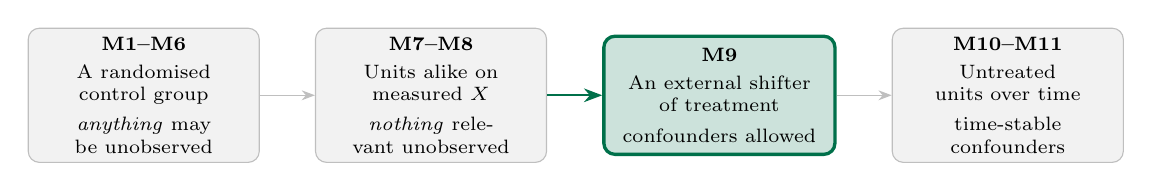
\begin{tikzpicture}[
    node distance=0.45cm and 0.7cm,
    box/.style={draw, rounded corners, minimum width=2.9cm, minimum height=1.5cm,
                font=\scriptsize, align=center, text width=2.7cm},
    active/.style={box, fill=sbgreen!20, draw=sbgreen, very thick},
    inactive/.style={box, fill=gray!10, draw=gray!50}
]
\node[inactive] (A) {\textbf{M1--M6}\\[2pt] A randomised control group\\[3pt] \emph{anything} may be unobserved};
\node[inactive, right=of A] (B) {\textbf{M7--M8}\\[2pt] Units alike on measured $X$\\[3pt] \emph{nothing} relevant unobserved};
\node[active, right=of B] (C) {\textbf{M9}\\[2pt] An external shifter of treatment\\[3pt] confounders allowed};
\node[inactive, right=of C] (D) {\textbf{M10--M11}\\[2pt] Untreated units over time\\[3pt] time-stable confounders};

\draw[-{Stealth}, gray!50] (A) -- (B);
\draw[-{Stealth}, thick, sbgreen] (B) -- (C);
\draw[-{Stealth}, gray!50] (C) -- (D);
\end{tikzpicture}
\end{center}

\bigskip

\begin{center}
\small M7--M8 needed \emph{nothing relevant unobserved}. Wen's overrides broke that.\\
Today the confounders stay. We find something that moves the rate and reaches bookings \textbf{only through the rate}.
\end{center}

\bigskip

\begin{center}
\scriptsize A cutoff that assigns treatment (regression discontinuity) is the same swap. It is in the notes, and not on Exam II.
\end{center}
\end{frame}

% ====================================================================
\begin{frame}{Today's Plan}

\begin{center}
\small
\begin{tabular}{rp{11.6cm}}
\toprule
\textbf{Minutes} & \\
\midrule
0--15 & \textbf{Reading and critique C5} --- a real excerpt; several flaws, to be \emph{ranked} \\
15--50 & \spinestep{Estimand:} the member-rate test and the number that settles it. \spinestep{Identification:} assignment versus receipt; four kinds of night; what the ratio estimates \\
60--110 & \spinestep{Identification under threat:} exclusion, controls, weak first stages; the candidate-instrument audit. \spinestep{Estimation:} 2SLS and the guard. The decision; consolidating M6--M9 \\
120--180 & \textbf{Workshop:} Wald ratios, weak first stages, coverage (prediction and hand calculation without AI) \\
\bottomrule
\end{tabular}
\end{center}

\bigskip

\textbf{Case:} Meridian Hotels, Meeting 9 (Releases 1--5). \quad \textbf{Next meeting:} Exam II (M6--M9).

\bigskip

\textbf{Reading:} technical notes for Meeting 9. Regression discontinuity and the fish-market example are there, and are not on Exam II.
\end{frame}

% ====================================================================
\begin{frame}{Critique C5: Rank the Flaws}

A real excerpt this time, with more than one problem. The five questions, then one more step.

\bigskip

\begin{enumerate}
    \item What is the claim?
    \item What causal question does the decision need?
    \item Who is the comparison group?
    \item What else could produce this pattern? Mechanism and \textbf{direction} of each bias.
    \item What would you do to find out?
\end{enumerate}

\bigskip

\textbf{Then rank the flaws} by how much each could change the decision. Most of them are M7--M8 ideas. Hand in your notes at minute 15.
\end{frame}

% ====================================================================
\section{The Estimand: The Member-Rate Test}
% ====================================================================

% [RELEASE R1 — narrative: the override problem, the test design, the proposal]
\begin{frame}{Wen's Problem, Continued}

M8 ended on an unlogged override: property managers overrule the RM system on about \textbf{8\% of nights}, and the reason is never recorded. DML's $-1.56$ rests on an assumption the logs cannot check.

\bigskip
\pause

\textbf{What Wen did next.} For six months the booking engine flipped a coin for every premium hotel-night:

\begin{itemize}
    \item \textbf{heads:} loyalty members see a \textbf{member rate 8\% below} the system's rate
    \item \textbf{tails:} they see the system's rate
\end{itemize}

Managers kept their override. On a heads night they could block the member rate; on a tails night they could apply it by hand.

\bigskip
\pause

\textbf{On her desk:} make the member rate permanent, portfolio-wide. Rate \textyen 800, variable cost \textyen 200.
\end{frame}

% ====================================================================
\begin{frame}{The Number That Decides It}

An 8\% member rate takes contribution per occupied room from \textyen 600 to \textyen 536.

\bigskip

The cut pays only if bookings rise by more than $600/536 - 1 = $ \textbf{11.9\%}.

\bigskip
\pause

\begin{alertblock}{Break-even elasticity}
\[
\eta^{*} = \frac{\ln(600/536)}{\ln(0.92)} = \mathbf{-1.35}
\]
\end{alertblock}

\bigskip

Every estimate today is an elasticity. The cut pays only if it lands \textbf{below $-1.35$}.

\medskip

M8's DML said $-1.56$ --- if the overrides did no harm.
\end{frame}

% ====================================================================
% [RELEASE R2 — the hand log; worksheet attempt before the next frame]
\begin{frame}{The Test Log}

One thousand premium hotel-nights from hotels where the coin was 50/50. Member bookings per night:

\bigskip

\begin{center}
\small
\begin{tabular}{llrr}
\toprule
\textbf{Coin} & \textbf{Member rate shown?} & \textbf{Nights} & \textbf{Mean bookings} \\
\midrule
Heads & yes & 350 & 64.0 \\
Heads & no  & 150 & 90.0 \\
Tails & yes & 50  & 40.0 \\
Tails & no  & 450 & 70.0 \\
\bottomrule
\end{tabular}
\end{center}

\bigskip

\textbf{In pairs:}
\begin{enumerate}\small
    \item bookings on nights the member rate was \emph{shown}, against nights it was not;
    \item bookings on \emph{heads} nights, against tails nights;
    \item the share of nights the rate was shown, heads against tails.
\end{enumerate}

Commit in writing --- does Wen roll it out?
\end{frame}

% ====================================================================
\begin{frame}{As Shown, Then As Assigned}

\textbf{As shown:}
\[
\frac{350(64) + 50(40)}{400} = 61.0, \qquad \frac{150(90) + 450(70)}{600} = 75.0, \qquad \text{difference} = \textcolor{warnred}{-14.0}
\]

\pause

\textbf{As assigned:}
\[
\bar Q_{\text{heads}} = \frac{350(64) + 150(90)}{500} = 71.8, \qquad
\bar Q_{\text{tails}} = \frac{50(40) + 450(70)}{500} = 67.0, \qquad \text{ITT} = \textcolor{sbgreen}{+4.8}
\]

\vspace{-0.4em}
\[
\text{shown: } \tfrac{350}{500} = 0.70 \text{ on heads}, \quad \tfrac{50}{500} = 0.10 \text{ on tails}, \qquad \text{first stage} = 0.60
\]

\pause

\begin{alertblock}{The ratio}
\[
\frac{4.8}{0.60} = \mathbf{8.0} \text{ bookings per night the coin switched the member rate on}
\]
\end{alertblock}

Same log. Opposite sign. The managers chose which heads to honour.
\end{frame}

% ====================================================================
\begin{frame}{Confounding by the Overrides}

\begin{center}
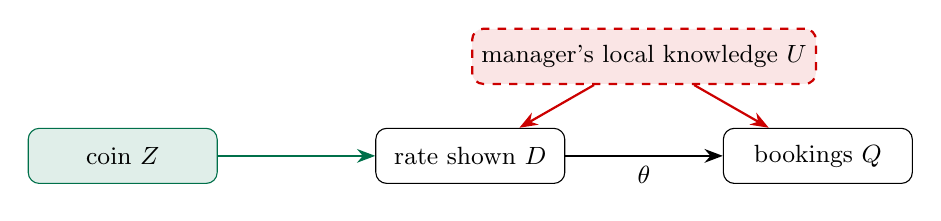
\begin{tikzpicture}[
    node distance=0.8cm and 2.0cm,
    v/.style={draw, rounded corners, minimum width=2.4cm, minimum height=0.7cm, font=\small},
    hid/.style={v, fill=warnred!10, draw=warnred, thick, dashed}
]
\node[v, fill=sbgreen!12, draw=sbgreen] (Z) {coin $Z$};
\node[v, right=of Z] (D) {rate shown $D$};
\node[v, right=of D] (Q) {bookings $Q$};
\node[hid, above=0.9cm of $(D)!0.5!(Q)$] (U) {manager's local knowledge $U$};
\draw[-{Stealth}, thick, sbgreen] (Z) -- (D);
\draw[-{Stealth}, thick] (D) -- node[below, font=\small] {$\theta$} (Q);
\draw[-{Stealth}, warnred, thick] (U) -- (D);
\draw[-{Stealth}, warnred, thick] (U) -- (Q);
\end{tikzpicture}
\end{center}

\medskip

Managers block the member rate on nights they expect to sell out (high $Q$) and apply it by hand on dead nights (low $Q$). ``Shown against not shown'' compares \textbf{different nights}.

\bigskip
\pause

\textbf{The coin has no arrow from $U$.} It was drawn by the booking engine, not by anyone who knew anything. Compare by the coin, not by what was shown.

\medskip

\begin{center}
\small $U$ is the M8 problem --- unrecorded, and moving both sides. The coin is how we get around it.
\end{center}
\end{frame}

% ====================================================================
\begin{frame}{Three Steps for an Instrument}

\begin{center}
\small
\begin{tabular}{p{2.8cm}p{9.8cm}}
\toprule
\spinestep{Estimand} & Two of them. The \textbf{ITT}: the effect of \emph{offering} the member rate, overrides and all. The \textbf{LATE}: the effect of the rate on nights the coin decided --- the compliers. Which one Wen needs depends on the programme she would actually run. \\[0.5em]
\spinestep{Identification} & The coin, within hotel $\times$ month (independence) --- for the ITT, that is all. For the LATE, also exclusion, monotonicity and relevance: claims about the booking engine and the managers. \\[0.5em]
\spinestep{Estimation} & The Wald ratio or 2SLS with the strata; SEs clustered by night; a first-stage guard written down before the ratio is computed. \\
\bottomrule
\end{tabular}
\end{center}

\bigskip

Randomisation buys the first line of identification. Everything after it has to be argued from the case.
\end{frame}

% ====================================================================
\section{Identification: Assignment Versus Receipt}
% ====================================================================

\begin{frame}{Two Effects of the Coin}

Your warm-up, in Meridian's terms:

\bigskip

\begin{center}
\footnotesize
\begin{tabular}{llrl}
\toprule
\textbf{Quantity} & \textbf{Definition} & \textbf{Hand log} & \textbf{Answers} \\
\midrule
ITT & $\E[Q \mid Z{=}1] - \E[Q \mid Z{=}0]$ & $4.8$ & ``offer it, overrides and all?'' \\
First stage & $\Prob(D{=}1 \mid Z{=}1) - \Prob(D{=}1 \mid Z{=}0)$ & $0.60$ & ``how often did the coin move the rate?'' \\
\bottomrule
\end{tabular}
\end{center}

\bigskip
\pause

\begin{itemize}
    \item Both are \textbf{causal} with no further assumption: the coin is random.
    \item The ITT is \textbf{diluted}. On 40\% of nights the coin changed nothing about the rate, so it measures the offer, not the price.
    \item Wen's proposal is about the \emph{price}. To get there, divide by how much the coin moved it.
\end{itemize}

\bigskip

\begin{center}
\small The ITT survives everything that goes wrong later today. Always report it.
\end{center}
\end{frame}

% ====================================================================
\begin{frame}{The Ratio and Its Interval}

\[
\widehat\theta_{\text{Wald}} = \frac{\text{ITT}}{\text{first stage}} = \frac{4.8}{0.60} = 8.0 \text{ bookings}
\]

\pause

When the first stage is precise, its noise is negligible and
\[
\SE(\widehat\theta_{\text{Wald}}) \;\approx\; \frac{\SE(\text{ITT})}{\text{first stage}} .
\]

\textbf{On the hand log}, with nightly bookings of standard deviation 20:
\[
\SE(\text{ITT}) = 20\sqrt{\tfrac{1}{500} + \tfrac{1}{500}} = 1.26, \qquad
\SE \approx \frac{1.26}{0.60} = 2.1, \qquad 8.0 \pm 4.1 = [3.9,\; 12.1] .
\]

\pause

On a base of 60 bookings, that is an elasticity from $-0.75$ to $-2.21$. \textbf{It straddles $-1.35$.} A thousand nights cannot decide; the full test will.

\medskip

\small Hotels share demand shocks on the same night: cluster by date, as in M8.
\end{frame}

% ====================================================================
\begin{frame}{Four Kinds of Night}

What would the rate shown have been under each coin?

\begin{center}
\small
\begin{tabular}{lccll}
\toprule
\textbf{Type} & \textbf{Tails} & \textbf{Heads} & \textbf{At Meridian} & \textbf{Share} \\
\midrule
Always-taker & shown & shown & dead night: manager applies it by hand & $0.10 = \Prob(D{=}1 \mid \text{tails})$ \\
Never-taker & not & not & near sell-out: manager blocks it & $0.30 = \Prob(D{=}0 \mid \text{heads})$ \\
Complier & not & shown & the coin decides & $0.60$ \\
Defier & shown & not & the manager does the opposite & assumed $0$ \\
\bottomrule
\end{tabular}
\end{center}

\bigskip
\pause

We never see a night's type, only its coin and what was shown:

\begin{itemize}\small
    \item heads and shown: a complier \emph{or} an always-taker
    \item tails and not shown: a complier \emph{or} a never-taker
\end{itemize}

\bigskip

The \textbf{shares} are still identified, from the two arms' rates. The types' outcomes are what the ratio untangles.
\end{frame}

% ====================================================================
\begin{frame}{What the Ratio Estimates}

The coin's effect on bookings, type by type:
\[
\text{ITT} = \pi_C\,\tau_C \;+\; \pi_A \cdot \underbrace{0}_{\text{rate unchanged}} \;+\; \pi_N \cdot \underbrace{0}_{\text{rate unchanged}} \;-\; \underbrace{\pi_D\,\tau_D}_{\text{no defiers}}
= \pi_C\,\tau_C ,
\]
and the first stage is $\pi_C$. So the ratio is the compliers' effect.

\pause
\medskip

\begin{alertblock}{Local average treatment effect (Imbens and Angrist 1994)}
\[
\frac{\text{ITT}}{\text{first stage}} \;=\; \E\bigl[Q(1) - Q(0) \;\big|\; \text{complier}\bigr] \;\equiv\; \text{LATE}
\]
\end{alertblock}

\pause
\medskip

\textbf{On the hand log:} $4.8 = 0.60 \times 8.0$. Complier nights book 60 without the member rate (the notes show how that is identified), so
\[
\frac{\ln(68/60)}{\ln(0.92)} = \textcolor{sbgreen}{-1.50} \qquad \text{past break-even, on complier nights.}
\]
\end{frame}

% ====================================================================
\begin{frame}{What Must Be True}

\begin{alertblock}{Four assumptions}
\begin{enumerate}
    \item \textbf{Independence.} The coin is as good as random (within the strata it was drawn in).
    \item \textbf{Exclusion.} The coin moves bookings \emph{only} through the rate shown.
    \item \textbf{Relevance.} The coin moves the rate: first stage $\neq 0$.
    \item \textbf{Monotonicity.} No defiers: the coin never pushes a night the other way.
\end{enumerate}
\end{alertblock}

\bigskip
\pause

Randomisation buys \textbf{only the first}. The other three are claims about the booking engine and the managers.

\medskip

Relevance is checkable in the data. Monotonicity is checkable in the institution. Exclusion is, in general, \textbf{checkable in neither}.
\end{frame}

% ====================================================================
\begin{frame}{The Assumptions, Sentence by Sentence}

From Wen's description of the test:

\bigskip

\begin{center}
\small
\begin{tabular}{p{6.6cm}p{6.4cm}}
\toprule
\textbf{The case says} & \textbf{Which buys} \\
\midrule
``The engine drew the coin within each hotel and month; resorts drew heads more often than airport hotels.'' & Independence, \emph{given} hotel $\times$ month. \\[0.5em]
``Heads changed one thing: the rate members were shown.'' & Exclusion. \\[0.5em]
``Managers honoured most heads and added the member rate on few tails.'' & Relevance: $0.70$ against $0.10$. \\[0.5em]
``A manager could block the member rate or add it by hand; none reversed the coin.'' & Monotonicity. \\
\bottomrule
\end{tabular}
\end{center}

\bigskip
\pause

\textbf{Hold onto the second sentence.} And note the first: the coin is random only \emph{within} hotel $\times$ month.
\end{frame}

% ====================================================================
\section{Identification Under Threat: When the Instrument Misbehaves}
% ====================================================================

% [RELEASE R3 — marketing's email; the zero-first-stage hotels]
\begin{frame}{The Email Nobody Mentioned}

Marketing confirms: on every heads night the engine also emailed \emph{``Members' Week at Meridian''} to members who had searched that hotel --- \textbf{whether or not the manager blocked the rate}.

\bigskip
\pause

Suppose the email alone adds 1.2 bookings on every heads night. Then
\[
\text{ITT} = 4.8 + 1.2 = 6.0, \qquad \frac{6.0}{0.60} = 10.0, \qquad \frac{\ln(70/60)}{\ln(0.92)} = \textcolor{warnred}{-1.85} .
\]

\pause

\begin{alertblock}{The ratio divides the violation by the first stage}
\[
\text{bias} = \frac{\text{direct effect of the coin}}{\text{first stage}} = \frac{1.2}{0.60} = 2.0 \text{ bookings}
\]
\end{alertblock}

\medskip

``Heads changed one thing'' was false. \textbf{Nothing in the test log shows it.}
\end{frame}

% ====================================================================
\begin{frame}{A Placebo for Exclusion}

Two hotels ran an old booking engine that \textbf{could not display} member rates. Their coin still flipped; the email still went out.

\bigskip

There the first stage is \textbf{zero by construction}. Any heads--tails gap in bookings is the email.

\begin{center}
\small
\begin{tabular}{lrrr}
\toprule
& \textbf{Heads} & \textbf{Tails} & \textbf{Gap} \\
\midrule
Old-engine hotels, 200 nights & 51.2 & 50.0 & $1.2$ \\
\bottomrule
\end{tabular}
\end{center}

\pause
\medskip

Corrected ratio: $(6.0 - 1.2)/0.60 = \textcolor{sbgreen}{8.0}$.

\bigskip
\pause

\begin{itemize}
    \item The correction assumes the email works the same in every hotel. It is a patch, not a proof.
    \item The clean fix is design: the next test sends the email on \textbf{both} sides of the coin.
    \item A group whose first stage is zero by construction is almost the only place exclusion can be tested.
\end{itemize}
\end{frame}

% ====================================================================
\begin{frame}{How Big Would the Email Have to Be?}

Let $a$ be the email's own effect per heads night. With the hand log (ITT $6.0$ with the email, first stage $0.60$, complier base $60$):
\[
\text{LATE} = \frac{6.0 - a}{0.60}, \qquad \eta = \frac{\ln\{(60 + \text{LATE})/60\}}{\ln 0.92}
\]

\begin{center}
\begin{tabular}{lrrrr}
\toprule
$a$ (bookings per heads night) & 0 & 1.2 & \textbf{1.71} & 2.4 \\
\midrule
Complier elasticity & $-1.85$ & $-1.50$ & $\mathbf{-1.35}$ & $-1.14$ \\
\bottomrule
\end{tabular}
\end{center}

\bigskip

\textbf{Break-even at $a = 1.71$.} The old-engine placebo measured $1.2$: the conclusion survives, by about half a booking a night. The data cannot say which column is true; the table prices the doubt.
\end{frame}

% ====================================================================
\begin{frame}{When the Offer Is the Policy}

Suppose the permanent programme would \textbf{keep} the ``Members' Week'' email.

\bigskip

\begin{itemize}
    \item Then the email's effect is \textbf{part of the policy}, not a bias. Exclusion is needed only to attribute an effect to the \emph{rate}.
    \item The estimand Wen needs is the \textbf{ITT} of the programme as it would run --- member rate, email and overrides together --- converted to contribution. The coin identifies it with nothing but independence.
    \item The email-corrected LATE answers a different question: the member rate \emph{without} the email.
\end{itemize}

\bigskip

\begin{block}{Step 1 decides step 2}
Name the programme before choosing the assumptions. The same data support two estimands, with two different identification burdens.
\end{block}
\end{frame}

% ====================================================================
\begin{frame}{Controls for Independence: Two Kinds of Hotel}

The coin was 70/30 at resorts and 30/70 at airport hotels. Resorts book more.

\begin{center}
\small
\begin{tabular}{lrrrrr}
\toprule
\textbf{Hotel} & \textbf{Nights} & \textbf{Heads} & \textbf{Tails mean} & \textbf{Heads mean} & \textbf{Ratio} \\
\midrule
Resort  & 500 & 350 & 80.0 & 84.8 & $4.8/0.60 = 8.0$ \\
Airport & 500 & 150 & 50.0 & 54.8 & $4.8/0.60 = 8.0$ \\
\bottomrule
\end{tabular}
\end{center}

\pause

\textbf{Pooled}, ignoring hotel type (first stage $0.60$ in both):
\[
\bar Q_{\text{heads}} = \frac{350(84.8) + 150(54.8)}{500} = 75.8, \quad
\bar Q_{\text{tails}} = \frac{150(80) + 350(50)}{500} = 59.0, \quad
\frac{16.8}{0.60} = \textcolor{warnred}{28.0}
\]

\pause

Heads nights are mostly resort nights. The coin is random only \emph{within} hotel type, so the comparison must be made there.

\medskip

\begin{center}
\textbf{Here controls buy independence, not precision.}
\end{center}
\end{frame}

% ====================================================================
\begin{frame}[shrink=8]{Two-Stage Least Squares Is FWL for the Ratio}

With the log rate as the treatment and strata $X$ as controls:

\vspace{-0.3em}
\begin{align*}
\text{first stage:} \quad \ln P &= \pi Z + X'\gamma + v \\
\text{reduced form:} \quad \ln Q &= \rho Z + X'\delta + u \qquad\qquad \widehat\theta_{\text{2SLS}} = \widehat\rho / \widehat\pi
\end{align*}

\vspace{-0.3em}
The M8 move, applied to the coin: residualise $Z$ on $X$, then
\[
\widehat\theta_{\text{2SLS}} = \frac{\sum_i \widetilde Z_i\, \ln Q_i}{\sum_i \widetilde Z_i\, \ln P_i}, \qquad \widetilde Z_i = Z_i - \widehat\E[Z \mid X_i] .
\]
Compare heads with tails \emph{within} strata, then take the ratio. $\widehat\theta$ is an elasticity directly.

\pause
\medskip

\begin{center}
\small
\begin{tabular}{lll}
\toprule
\textbf{Control} & \textbf{Status} & \textbf{Why} \\
\midrule
Hotel $\times$ month & \textcolor{sbgreen}{required} & sets the coin's probability \\
The 47 demand signals & optional & predict bookings: shrink the SE \\
Manager overrode? Rate shown? & \textcolor{warnred}{never} & caused by the coin (M7's bad controls) \\
\bottomrule
\end{tabular}
\end{center}

\small Run the two stages by hand for intuition only: the second-stage SE treats the fitted rate as data and is wrong. Take the SE from the IV routine.
\end{frame}

% ====================================================================
% [RELEASE R4 — full test description; collect predictions before the ladder]
\begin{frame}{Predict Before You Look}

The full test: 80 hotels, 182 nights, \textbf{14{,}560 premium hotel-nights}. Coin probability set by hotel $\times$ month.

\bigskip

\textbf{In pairs, write down three elasticities:}

\bigskip

\begin{enumerate}
    \item the Wald ratio pooled over all hotels, no controls
    \item 2SLS with hotel $\times$ month strata
    \item 2SLS with strata and the 47 signals, corrected for the email using the old-engine hotels
\end{enumerate}

\bigskip

Against the break-even $-1.35$, which ones roll out the member rate?

\bigskip

\begin{center}
\small Commit before the next slide.
\end{center}
\end{frame}

% ====================================================================
\begin{frame}{The Ladder}

\begin{center}
\small
\begin{tabular}{lr}
\toprule
\textbf{Comparison} & \textbf{Elasticity (SE)} \\
\midrule
Shown against not shown, no controls & \textcolor{warnred}{\NUM{$+0.35$}{sim meridian-iv v1: OLS of ln Q on ln P, test nights, no controls}} \\
Wald ratio, pooled, no controls & \textcolor{warnred}{\NUM{$-3.10$}{sim meridian-iv v1: Wald on ln Q and ln P, strata ignored}} \\
2SLS, hotel $\times$ month & \NUM{$-1.86$ (0.15)}{sim meridian-iv v1: 2SLS with hotel x month FE; date-clustered SE} \\
2SLS, strata $+$ 47 signals & \NUM{$-1.84$ (0.08)}{sim meridian-iv v1: 2SLS with FE and signals; date-clustered SE} \\
\midrule
\textit{(today's destination: email-corrected)} & \textcolor{sbgreen}{\NUM{$-1.55$ (0.08)}{sim meridian-iv v1: 2SLS with FE and signals, reduced form net of the old-engine ITT; SE}} \\
\bottomrule
\end{tabular}
\end{center}

\pause

\small
\begin{itemize}
    \item The signals barely moved the estimate and halved its SE: the coin was already random within strata.
    \item The email correction moved it \textbf{more than any control did} --- the only step that addresses an assumption.
\end{itemize}
\end{frame}

% ====================================================================
\begin{frame}{Weak Instruments}

In the 12 city-centre hotels, managers overrode the coin almost always: the member rate was shown on 15\% of heads nights and 10\% of tails nights. 200 nights per arm.

\begin{center}
\small
\begin{tabular}{lrr}
\toprule
& \textbf{Hand log} & \textbf{City hotels} \\
\midrule
First stage & $0.70 - 0.10 = 0.60$ & $0.15 - 0.10 = 0.05$ \\
SE of first stage & $\sqrt{\tfrac{0.7(0.3) + 0.1(0.9)}{500}} = 0.024$ & $\sqrt{\tfrac{0.15(0.85) + 0.1(0.9)}{200}} = 0.033$ \\
$F = (\text{first stage} / \text{SE})^2$ & 600 & \textcolor{warnred}{2.3} \\
SE of the ratio $\approx \SE(\text{ITT}) / \text{first stage}$ & $1.26 / 0.60 = 2.1$ & $2.0 / 0.05 = \textcolor{warnred}{40}$ \\
Email bias $= 1.2 / \text{first stage}$ & 2.0 & \textcolor{warnred}{24} \\
\bottomrule
\end{tabular}
\end{center}

\pause

\textbf{Weak and slightly invalid is the worst combination.} The violation is multiplied by 20, and the interval is too wide for anyone to notice.

\medskip

And the approximation itself fails: with a weak first stage the ratio's distribution is heavy-tailed, drifts toward the ``as shown'' answer, and its nominal 95\% interval covers far less (the workshop measures how much).
\end{frame}

% ====================================================================
\begin{frame}{The First-Stage Guard}

\begin{block}{Written down before the estimate is computed}
\begin{enumerate}
    \item Report the first stage and its $F$ statistic, clustered as the estimate will be.
    \item If $F < 10$, \textbf{do not report the ratio}. Report the ITT and the first stage separately.
    \item If $F$ is above 10 but not far above, use an interval that is valid for weak instruments (Anderson--Rubin; in the notes). $F > 10$ is a floor, not a certificate (Lee et al., 2022).
\end{enumerate}
\end{block}

\pause
\smallskip

\begin{center}
\small
\begin{tabular}{lrl}
\toprule
& \textbf{First-stage $F$} & \textbf{Report} \\
\midrule
City hotels & 2.3 & ITT and first stage only \\
Full test, strata $+$ signals & \NUM{410}{sim meridian-iv v1: date-clustered first-stage F} & 2SLS elasticity and interval \\
\bottomrule
\end{tabular}
\end{center}

\smallskip

Like M5's frozen list, the guard is a commitment made \textbf{before} the answer is visible. A threshold chosen after seeing the estimate guards nothing.

\end{frame}

% ====================================================================
% [RELEASE R5 — candidate-instrument worksheet; answers on the next frame after the attempt]
\begin{frame}{Candidate-Instrument Audit}

Analysts across the group propose other instruments for the rate. \textbf{In pairs:} mark each assumption \textcolor{sbgreen}{\checkmark}, \textcolor{warnred}{$\times$} or ?, with one reason.

\bigskip

\begin{center}
\small
\begin{tabular}{p{5.2cm}cccc}
\toprule
\textbf{Candidate} & \textbf{Relevance} & \textbf{Independence} & \textbf{Exclusion} & \textbf{Monotonicity} \\
\midrule
A competitor's rate the same night & & & & \\[0.4em]
Rainfall in the city & & & & \\[0.4em]
Nights the RM system was down and rates froze at yesterday's level & & & & \\[0.4em]
Which revenue manager was on shift & & & & \\[0.4em]
The member-rate coin & & & & \\
\bottomrule
\end{tabular}
\end{center}

\bigskip

\begin{center}
\small Commit before the next slide.
\end{center}
\end{frame}

% ====================================================================
\begin{frame}{The Audit, Answered}

\begin{center}
\scriptsize
\begin{tabular}{p{2.9cm}p{2.1cm}p{2.4cm}p{2.6cm}p{2.3cm}}
\toprule
\textbf{Candidate} & \textbf{Relevance} & \textbf{Independence} & \textbf{Exclusion} & \textbf{Monotonicity} \\
\midrule
Competitor's rate & \textcolor{sbgreen}{\checkmark} the system reacts to it & \textcolor{warnred}{$\times$} competitors see the same demand & \textcolor{warnred}{$\times$} guests compare rates directly & ? \\[0.4em]
Rainfall & ? weak & \textcolor{sbgreen}{\checkmark} & \textcolor{warnred}{$\times$} rain moves demand itself & ? \\[0.4em]
System outage & \textcolor{sbgreen}{\checkmark} & ? outages cluster at peak load & \textcolor{sbgreen}{\checkmark} plausible & \textcolor{warnred}{$\times$} freezing raises some rates, lowers others \\[0.4em]
Manager on shift & \textcolor{sbgreen}{\checkmark} managers differ & \textcolor{sbgreen}{\checkmark} if the rota is set in advance & ? managers also upsell and handle groups & ? strict on weddings, lenient on conferences \\[0.4em]
Member-rate coin & \textcolor{sbgreen}{\checkmark} 0.60 & \textcolor{sbgreen}{\checkmark} within strata & \textcolor{warnred}{$\times$} the email --- fixable & \textcolor{sbgreen}{\checkmark} no reversals \\
\bottomrule
\end{tabular}
\end{center}

\pause
\medskip

Most candidates fail on \textbf{exclusion}, and exclusion cannot be tested in general. The coin passes because someone \emph{designed} it --- and even the designed instrument failed once.
\end{frame}

% ====================================================================
\begin{frame}{Whose Elasticity Is This?}

\begin{center}
\small
\begin{tabular}{lrll}
\toprule
\textbf{Nights} & \textbf{Share} & \textbf{Bookings seen} & \textbf{What the coin tells us} \\
\midrule
Always-takers (dead nights) & 0.10 & 40 with the member rate & nothing: cut regardless \\
Compliers & 0.60 & 60 without, 68 with & elasticity $-1.50$ \\
Never-takers (near sell-out) & 0.30 & 90 without the member rate & nothing: rate never changed \\
\bottomrule
\end{tabular}
\end{center}

\pause
\medskip

\begin{itemize}
    \item The ratio is the elasticity of \textbf{nights managers let the coin decide}. On nights near sell-out a cut cannot sell rooms that do not exist.
    \item It is local in size, too: an 8\% cut, not the 30\% that M8's formula suggested.
    \item M8's DML averaged over nights where the \emph{system} left rates room to vary. Today's LATE averages over \emph{compliers}. Different nights: a disagreement is not by itself a contradiction.
\end{itemize}

\bigskip

\begin{center}
\textbf{Say whose elasticity you estimated.}
\end{center}
\end{frame}

% ====================================================================
\section{The Decision}
% ====================================================================

\begin{frame}{Wen's Table}

\begin{center}
\scriptsize
\begin{tabular}{llrl}
\toprule
\textbf{Method} & \textbf{What it estimates} & \textbf{Elasticity} & \textbf{Verdict} \\
\midrule
Shown against not shown & nothing causal & \NUM{$+0.35$}{sim v1: OLS, no controls} & \textcolor{warnred}{never cut} \\
M8's DML, test nights & variance-weighted, if no unrecorded confounder & \NUM{$-1.58$}{sim v1: cross-fitted PLR on test nights} & roll out \\
Wald ratio, pooled & nothing: strata mixed & \NUM{$-3.10$}{sim v1: pooled Wald} & \textcolor{warnred}{roll out, loudly} \\
2SLS, strata $+$ signals & LATE plus the email's effect & \NUM{$-1.84$}{sim v1: 2SLS} & roll out \\
2SLS, email-corrected & LATE on complier nights & \textcolor{sbgreen}{\NUM{$-1.55$}{sim v1: corrected 2SLS}} & \textcolor{sbgreen}{roll out there} \\
City hotels & not reported: $F = 2.3$ & --- & ITT only \\
\bottomrule
\end{tabular}
\end{center}

\pause
\medskip

\small Four methods say ``roll out''. They are \textbf{not} ordered worst to best, and only one of them says \emph{where}. The simulation's true elasticities are released in the workshop, not here.
\vspace{1.2em}
\end{frame}

% ====================================================================
\begin{frame}{The Recommendation}

At the hand log's $-1.50$, an 8\% member rate on complier nights:
\[
\text{bookings} \times 0.92^{-1.50} = \times 1.133, \qquad
\frac{536 \times 1.133}{600} - 1 = \textcolor{sbgreen}{+1.2\%} \text{ of contribution}
\]
At the email-inflated $-1.85$ it gives $+4.2\%$: the number marketing will quote.

\pause

\begin{block}{To Wen}
Switch the member rate on for nights managers now leave to the system and that are not forecast to sell out; the full test puts their elasticity at \NUM{$-1.55$}{sim v1: corrected 2SLS} $\pm$ $1.96 \times$ \NUM{0.08}{sim v1: SE}, past $-1.35$, worth \NUM{$+1.7\%$}{536 x 0.92\^{}(theta-hat) / 600 - 1 at the corrected 2SLS} of contribution. Do not extend it to peak nights. Rerun with the email on both arms, and test the city hotels with a coin managers cannot override.
\end{block}

\pause

The margin is thin. The case for the rollout rests on the \textbf{interval}, on \textbf{whose nights} it describes, and on a correction that assumes the email works the same everywhere.
\end{frame}

% ====================================================================
\begin{frame}{Key Takeaways}

\begin{itemize}
    \item \spinestep{Estimand.} Two candidates: the ITT of the offer, and the LATE of the rate on complier nights. Name the programme first --- if the email continues, it is part of the policy.
    \item \spinestep{Identification.} Compare by what was assigned, not by what was received: shown vs not gave $-14$; the coin gave $+4.8$. Randomisation buys only independence; exclusion, monotonicity and relevance are claims about the institution.
    \item \spinestep{Estimation.} ITT over first stage; 2SLS with the strata that set the coin's probability; SEs by night. The ratio magnifies a direct effect and sampling noise alike: guard before you divide.
    \item \textbf{Price the doubt.} The email would have to add 1.71 bookings a night to overturn the rollout.
    \item \textbf{Every IV estimate is local.} Say whose nights, and how large a change.
\end{itemize}

\bigskip

\textbf{Next time:} Exam II (M6--M9), then units observed before and after --- difference-in-differences.
\end{frame}

% ====================================================================
\begin{frame}{Consolidating M6--M9 for Exam II}

Four questions --- the second half of the course so far:

\begin{center}
\footnotesize
\begin{tabular}{lll}
\toprule
\textbf{Meeting} & \textbf{Question} & \textbf{The object to be able to compute} \\
\midrule
M6 & Which list, under constraints? & $v_i$; cap and ratio rankings; $\lambda^*$; reserve $z\sigma_C$ \\
M7 & Can logs replace an experiment? & standardisation; IPW; overlap, trimming; ATT vs ATE \\
M8 & How must $X$ enter? & FWL; cross-fitting; the product of errors; variance weights \\
M9 & What if $U$ moved the treatment? & ITT; first stage; Wald/LATE; four assumptions; $F$ guard \\
\bottomrule
\end{tabular}
\end{center}

\bigskip

Every exam question has a \textbf{number that decides it}. Find it first, then ask which comparison produced it --- and for whom.

\medskip

\begin{center}
\small Exam II contains no regression-discontinuity items.
\end{center}
\end{frame}

% ====================================================================
\begin{frame}[shrink=6]{Workshop: Wald Ratios, Weak First Stages, Coverage}

\small Prediction and hand calculation without AI; AI allowed, with disclosure, in the implementation step.
\normalsize

The member-rate test, simulated with known elasticities. Sixty minutes, scripted.
\vspace{-0.3em}

\begin{center}
\scriptsize
\begin{tabular}{rlp{8.4cm}}
\toprule
\textbf{Min} & \textbf{Slot} & \textbf{Prompt} \\
\midrule
7  & Predict & As the first stage falls from 0.60 to 0.05, what happens to the ratio's centre and to its interval's coverage? \\
10 & Hand calculation & ITT, first stage, ratio and SE for the printed 40-night log; apply the guard. \\
5  & Demonstration & 2SLS with hotel $\times$ month strata: $F$, estimate, date-clustered SE. \\
15 & Implement & Your 2SLS with the signals; the email correction from the old-engine hotels. \\
10 & \textbf{Perturbation} & Let managers override more: first stage 0.60, 0.30, 0.10, 0.05. At each, 500 simulated tests; record the median ratio and the coverage of the nominal 95\% interval. \\
8  & \textbf{Comparison} & Corrected 2SLS, uncorrected 2SLS and M8's DML against the simulation's true complier elasticity \emph{and} its true average elasticity. \\
5  & Interpret & One sentence to Wen: which number goes in the memo, and for which nights. \\
\bottomrule
\end{tabular}
\end{center}

\small \textbf{Consolidation (3 min):} with a weak first stage the ratio's distribution is heavy-tailed, its centre drifts toward the ``as shown'' answer and its interval covers far less than 95\% --- hence the guard. The corrected 2SLS recovers the \emph{complier} elasticity, not the average one: it answers for compliers only.
\end{frame}

\end{document}
